%# -*- coding:utf-8 -*-
\section{研究背景}

\begin{frame}
\frametitle{冠心病病理}
\begin{itemize}
  \item 冠心病病理: 
  \begin{enumerate}[A]
    \item 由于冠状动脉中的血流受阻,导致自受阻位置以下心肌长期缺氧,最终使其坏死
    \item 受阻的冠状动脉内部情况,斑块固着于血管内壁,致使血管横截面积明显缩小,血流受阻
  \end{enumerate}
\end{itemize}
\begin{figure}[t]
\centering
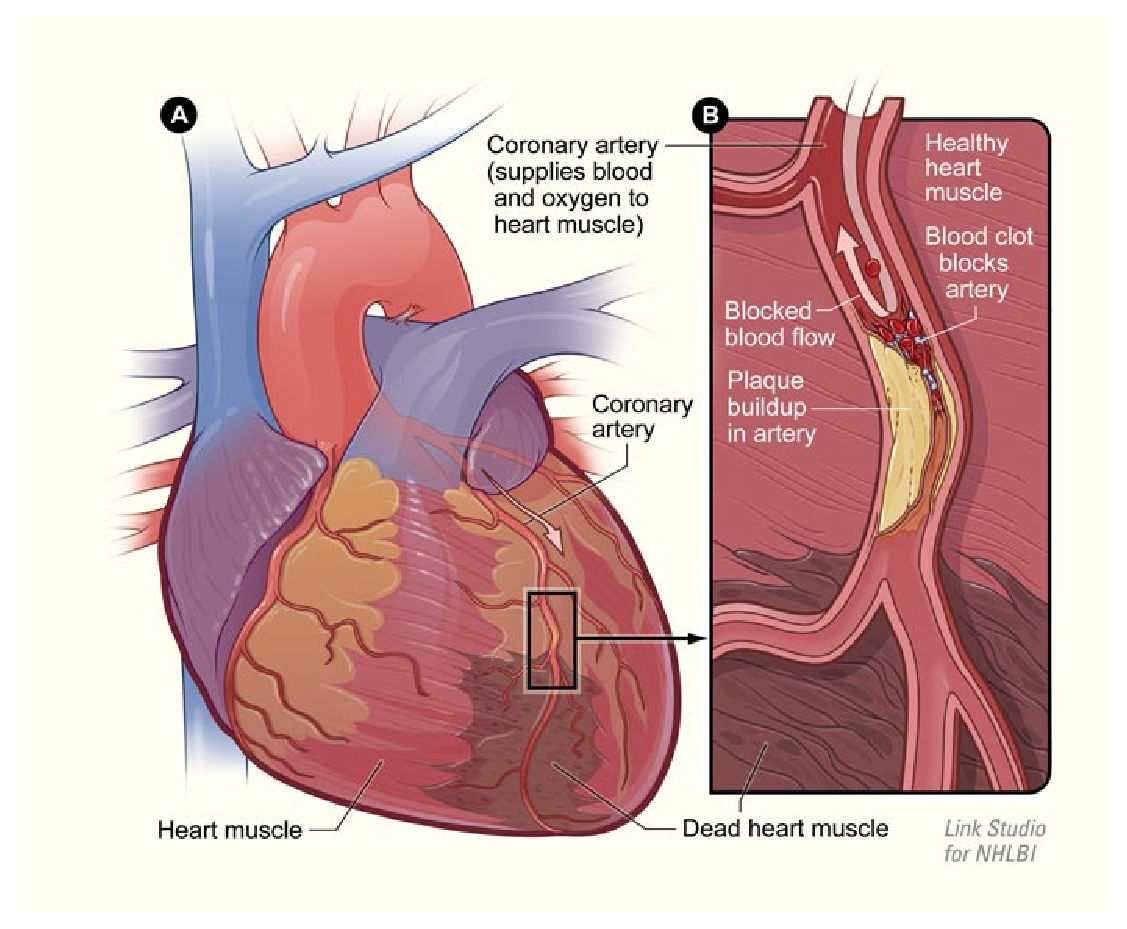
\includegraphics[height=130pt]{../../Figures/background/heart_attack_large.eps}
\caption[冠心病病理]{图片来自:\url{http://www.nhlbi.nih.gov/index.html}}
% \label{fig:heart_attack}
\end{figure}
\end{frame}

\begin{frame}
\frametitle{冠状动脉介入术}
\begin{columns}[onlytextwidth]
\begin{column}{0.4\textwidth}
\begin{figure}[t]
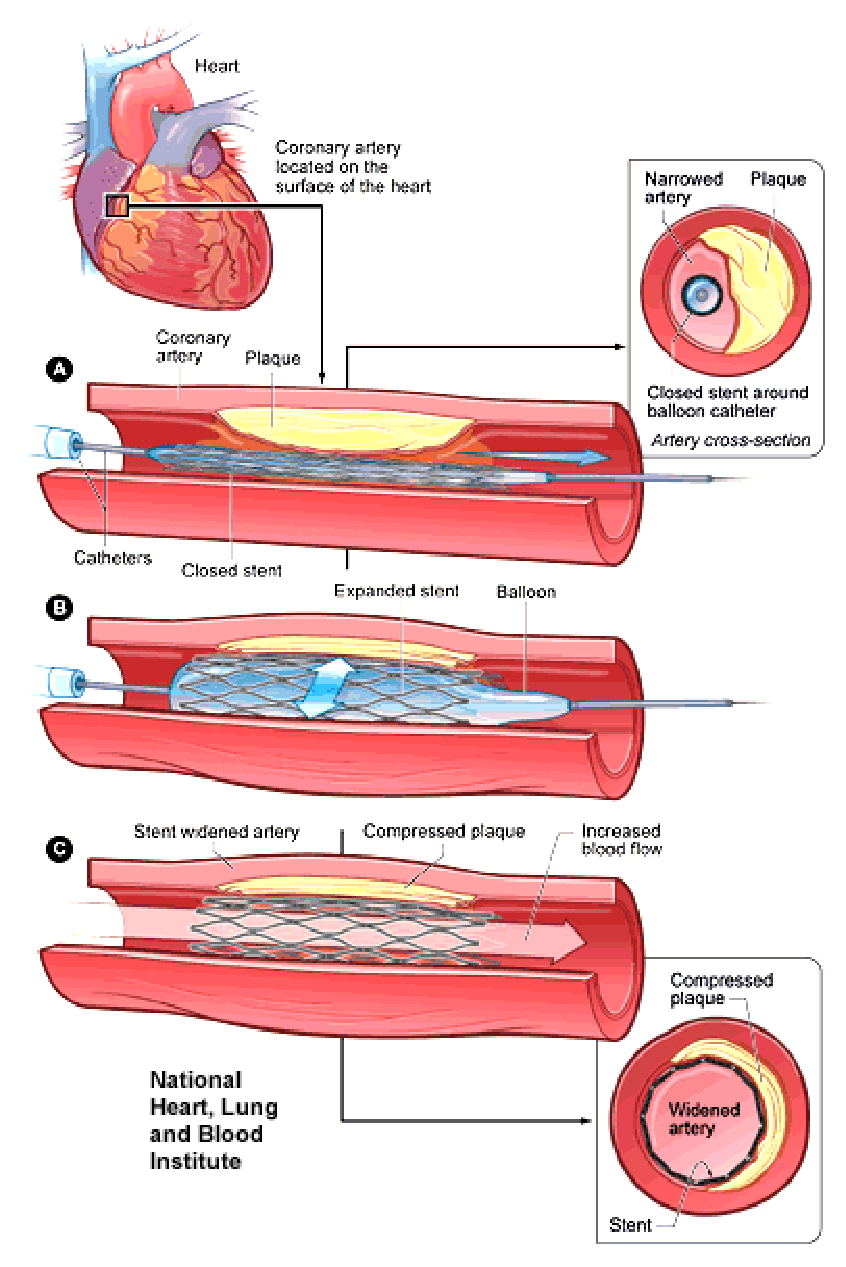
\includegraphics[height=170pt]{../../Figures/background/phauthuatmachmau_stent.eps}
\caption[冠状动脉介入术]{图片来自:\url{http://www.nhlbi.nih.gov/index.html}}
\end{figure}
\end{column}
\begin{column}{0.5\textwidth}
\begin{itemize}
\item \textbf{冠状动脉介入术}: minimally invasive procedure to open up blocked coronary arteries
\item \textbf{主要步骤}:
\begin{enumerate}[A]
\item \footnotesize{将载有收缩态气囊的导管沿主动脉送至病灶位置}
\item \footnotesize{通过导管向气囊注入空气,迫使包被在气囊外的支架向周围血管壁扩张}
\item \footnotesize{当血管壁扩张所得到的血管横截面达到恢复血运的程度时,再通过导管抽出气囊内部的空气使其收缩后撤出人体,留下扩张好的支架以保持血运流畅}
\end{enumerate}
\end{itemize}
\end{column}
\end{columns}
\end{frame}

\begin{frame}

\end{frame}

\begin{frame}

\end{frame}